\documentclass[a4paper,11pt,twocolumn]{article}

\usepackage{amsmath}
\usepackage{amssymb}
\usepackage[english]{babel}
\usepackage[style=ieee,backend=bibtex]{biblatex}
	\bibliography{references.bib}
\usepackage{booktabs}
\usepackage[font={small},labelfont=sc]{caption}
\usepackage{helvet}
\usepackage[hidelinks]{hyperref}
\usepackage{geometry}
\usepackage{fancyhdr}
\usepackage{float}
\usepackage[symbol]{footmisc}
\usepackage{graphicx}
\usepackage[latin1]{inputenc}
\usepackage{listings}
\usepackage{mathtools}
\usepackage{microtype}
\usepackage{nomencl}
	\setlength{\nomitemsep}{0pt}
	\makenomenclature
\usepackage{siunitx}
\usepackage{threeparttable}
\usepackage{tikz,pgfplots}
    \pgfplotsset{compat=1.15,set layers}
	\usetikzlibrary{angles}
	\usetikzlibrary{calc}
    \usetikzlibrary{external}
    	\tikzexternalize[prefix=tikz/]
	\usetikzlibrary{pgfplots.groupplots}
	\usetikzlibrary{positioning}
	\usetikzlibrary{shapes.misc}
    \usepgfplotslibrary{fillbetween}
\usepackage{titling}
\usepackage{xspace}

\renewcommand{\sfdefault}{phv}
\renewcommand{\familydefault}{\sfdefault}

\newcommand{\Matlab}{\textsc{Matlab}\textsuperscript{\textregistered}\xspace}
\newcommand{\sse}{\textsc{sse}\xspace}
\newcommand{\Sse}{\textsc{Sse}\xspace}

\title{Controller Design in \Matlab}
\author{Z0996690}
\date{\today}

\pagestyle{fancy}
\fancyhf{}
\lhead{
\includegraphics[width=0.1\textwidth]{img/Durham.png}}
\chead{\thetitle}
\rhead{\theauthor}
\cfoot{\thepage}

% Listings preamble
\definecolor{codegreen}{rgb}{0,0.6,0}
\definecolor{codegray}{rgb}{0.5,0.5,0.5}
\definecolor{codepurple}{rgb}{0.58,0,0.82}
\definecolor{backcolour}{rgb}{0.95,0.95,0.92}

\lstdefinestyle{mystyle}{
    backgroundcolor=\color{backcolour},
    commentstyle=\color{codegreen},
    keywordstyle=\color{magenta},
    numberstyle=\tiny\color{codegray},
    stringstyle=\color{codepurple},
    basicstyle=\ttfamily\footnotesize,
    breakatwhitespace=false,
    breaklines=true,
    captionpos=b,
    keepspaces=true,
    numbers=left,
    numbersep=5pt,
    showspaces=false,
    showstringspaces=false,
    showtabs=false,
    tabsize=2
}

\renewcommand{\thefootnote}{\fnsymbol{footnote}}

\begin{document}

% Title page.
\begin{titlepage}
    \centering
    \vspace*{\fill}
    
\includegraphics[width=0.5\textwidth]{img/Durham.png}\\
    \vspace*{\fill}
    \LARGE\thetitle\\
    \vskip0.2em
    \large Level 3 Control and Signal Processing\\
    \vskip0.4em
    \large\theauthor\\
    \vskip0.4em
    \large\thedate\\
    \vspace*{\fill}
\end{titlepage}

% Abstract
\twocolumn[{%
\begin{@twocolumnfalse} \centering
    \renewcommand{\abstractname}{\large Abstract}
    \begin{abstract}
        This report describes the design of two controllers for an industrial plant process in \Matlab. Each controller was designed to meet a different performance specification.
    \end{abstract}
    \vskip\parsep
\end{@twocolumnfalse}
}]

% Acronyms
% Lowercase latin
\nomenclature[1s]{$s$}{Laplace domain variable\hfill[\si{\radian\per\second}]}
\nomenclature[1t]{$t$}{Time domain variable\hfill[\si{\second}]}

% Lowercase greek
\nomenclature[2f]{$\zeta$}{Damping factor}
\nomenclature[2f]{$\omega_n$}{Natural frequency}

% Uppercase latin
\nomenclature[4G]{$G$}{Industrial plant process transfer function}
\nomenclature[4Gc]{$G_c$}{Controller transfer function}
\nomenclature[4L]{$\mathcal{L}$}{Laplace transform operator}
\nomenclature[4M0]{$M_0$}{Peak overshoot\hfill[\si{\%}]}
\nomenclature[4SSE]{$\mathit{SSE}$}{Steady state error}
\nomenclature[4Tr]{$T_r$}{Eighty percent rise time\hfill[\si{\second}]}
\nomenclature[4Ts]{$T_s$}{Two percent settling time\hfill[\si{\second}]}

% Uppercase greek
\printnomenclature

\section{Introduction}
\section{Background}

Figure~\ref{fig:closed} illustrates a closed loop system. The controller is designed to drive the output $y(s)$ of the plant process to the desired output $r(s)$ by minimising the error $e(s)$.

\begin{figure}[h]
	\centering
	\footnotesize
	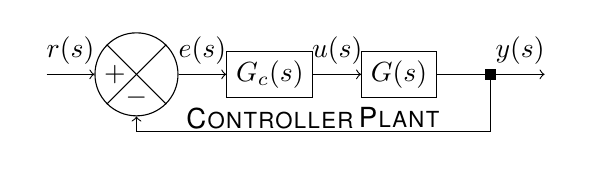
\begin{tikzpicture}[node distance=0.05\textwidth and 0.05\textwidth]
		\node (desire) {};
		\node [draw,right=of desire,circle,minimum size=3em] (sum) {};
			\draw (sum.north west) -- (sum.south east);
			\draw (sum.north east) -- (sum.south west);
		\node [draw,right=of sum,rectangle] (controller) {$G_c(s)$};
		\node [draw,right=of controller,rectangle] (plant) {$G(s)$};
		\node [fill,right=of plant,rectangle,inner sep=2pt] (branch) {};
		\node [right=of branch] (output) {};
		\node [below=of branch.center] (feedback1) {};
		\node [below=of sum.center] (feedback2) {};

		\draw [->] (desire) -- (sum);
		\draw [->] (sum) -- (controller);
		\draw [->] (controller) -- (plant);
		\draw [->] (plant) -- (output);
		\draw [->] (branch) -- (feedback1.center) -- (feedback2.center) -- (sum);

		\node [anchor=west] at (sum.west) {$+$};
		\node [anchor=south] at (sum.south) {$-$};

		\node [anchor=south west] at (desire) {$r(s)$};
		\node [anchor=south] at ($(sum.east)!0.5!(controller.west)$) {$e(s)$};
		\node [anchor=south] at ($(controller.east)!0.5!(plant.west)$) {$u(s)$};
		\node [anchor=south east] at (output) {$y(s)$};

		\node [anchor=north] at (controller.south) {\textsc{Controller}};
		\node [anchor=north] at (plant.south) {\textsc{Plant}};
	\end{tikzpicture}
	\caption{Block diagram of the closed loop system.}
	\label{fig:closed}
\end{figure}

For low frequency applications the controller performance can be characterised by analysing the step response.

Percentage overshoot $M_0$ is the the peak response in proportion to the final output value and is soley dependent on the damping factor $\zeta$ for second order systems:
\begin{equation}
	M_0 = \exp\left(-\frac{\pi\zeta}{\sqrt{1-\zeta^2}}\right)
	\footnote{Equality holds for second order systems only, but may be used to approximate higher order characteristics.}
\end{equation}
The settling time $T_s$ of the controller is the time for the output oscillations to decay to within some margin of the final value: \SI{2}{\%} is used in this report. Settling time is also dependent on the natural frequency $\omega_n$:
\begin{equation}
	T_s = -\frac{\ln\left(2\%\right)}{\zeta\omega_n} \approx \frac{4}{\zeta\omega_n}
	\footnotemark[\value{footnote}]
\end{equation}
The rise time of the controller is the time for the output to transition from \SIrange{10}{90}{\%} of the final value:
\begin{equation}
	T_r = \frac{\ln\left(90\%/10\%\right)}{\zeta\omega_n} \approx \frac{2.2}{\zeta\omega_n}
	\footnotemark[\value{footnote}]
\end{equation}
These three parameters are typically specified as upper bounds and constitute the dynamic specification.

In controller design there is a tradeoff between the dynamic specification and the steady state error. The steady state error is defined as follows:
\begin{equation}
	\mathit{SSE} \coloneqq \lim_{t\rightarrow\infty}{e(t)}
\end{equation}

One of the most common types of controller in industry is the PID controller, which can be easily implemented using microcontrollers.

\begin{figure}[h]
	\centering
	\footnotesize
	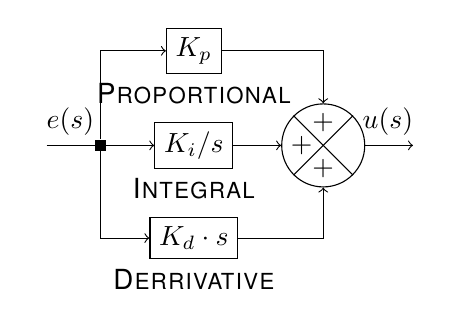
\begin{tikzpicture}[node distance=0.05\textwidth and 0.05\textwidth]
		\node (error) {};
		\node [fill,right=of error,rectangle,inner sep=2pt] (branch) {};
		\node [draw,right=of branch,rectangle] (i) {${K_i}/{s}$};
		\node [draw,above=of i,rectangle] (p) {$K_p$};
		\node [draw,below=of i,rectangle] (d) {${K_d}\cdot{s}$};
		\node [draw,right=of i,circle,minimum size=3em] (sum) {};
			\draw (sum.north west) -- (sum.south east);
			\draw (sum.north east) -- (sum.south west);
		\node [right=of sum] (output) {};

		\draw [->] (branch) |- (p);
		\draw [->] (error) -- (i);
		\draw [->] (branch) |- (d);
		\draw [->] (p) -| (sum);
		\draw [->] (i) -- (sum);
		\draw [->] (d) -| (sum);
		\draw [->] (sum) -- (output);

		\node [anchor=north] at (sum.north) {$+$};
		\node [anchor=west] at (sum.west) {$+$};
		\node [anchor=south] at (sum.south) {$+$};

		\node [anchor=south west] at (error) {$e(s)$};
		\node [anchor=south east] at (output) {$u(s)$};

		\node [anchor=north] at (p.south) {\textsc{Proportional}};
		\node [anchor=north] at (i.south) {\textsc{Integral}};
		\node [anchor=north] at (d.south) {\textsc{Derrivative}};
	\end{tikzpicture}
	\caption{Block diagram of a PID controller}
	\label{fig:pid}
\end{figure}

\begin{figure}[h]
	\centering
	\footnotesize
	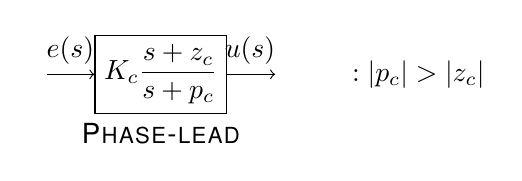
\begin{tikzpicture}[node distance=0.05\textwidth and 0.05\textwidth]
		\node (error) {};
		\node [draw,right=of error,rectangle] (C) {$K_c\dfrac{s+z_c}{s+p_c}$};
		\node [right=of C] (output) {};

		\draw [->] (error) -- (C);
		\draw [->] (C) -- (output);

		\node [anchor=south west] at (error) {$e(s)$};
		\node [anchor=south east] at (output) {$u(s)$};
		\node [right=of output] {$:|p_c| > |z_c|$};

		\node [anchor=north] at (C.south) {\textsc{Phase-lead}};
	\end{tikzpicture}
	\caption{Block diagram of a phase-lead controller.}
	\label{fig:pid}
\end{figure}

\section{Specification}

The transfer function for the industrial plant process $G(s)$ was given as follows:
\begin{equation} \label{eq:G}
	G(s) = \frac{s + 1}{s(s^2 + 4s + 5)}
\end{equation}
The transfer function $G_c(s)$ for the two controllers was chosen to meet the system performance specification detailed in Table~\ref{tab:spec}.

\begin{table}[h]
	\centering
	\footnotesize
	\begin{threeparttable}
		\caption{System perfomance specification.}
		\label{tab:spec}
		\begin{tabular}{@{}crrrr@{}}
			\toprule
			\textsc{System} &
				$M_0$[\%] &
				$T_r$[\si{\second}] &
				$T_{2\%}$[\si{\second}] &
				$SSE$[\%] \\
			\cmidrule(r){1-1}\cmidrule(l){2-5}
			1 &  5 & 1.0 &   4 & --- \\
			2 & 20 & 0.5 & --- &   5 \\
			\bottomrule
		\end{tabular}
	\end{threeparttable}
\end{table}

\section{Design}

\begin{figure}[h]
	\centering
	\footnotesize
	\begin{tikzpicture}
		\begin{axis}[
			axis lines=middle,
			xmin=-2.1,xmax=0.5,
			ymin=-5,ymax=5,
			xlabel={$\Re(s)$},ylabel={$\Im(s)$},
		]
			\addplot [thick,cyan]
				table [x={re1}, y={im1}] {data/rlocus.dat}
				node [draw,black,cross out,inner sep=1.7pt]
					at (current plot begin) {}
				node [draw,black,circle,inner sep=1.7pt]
					at (current plot end) {};
			\addplot [thick,cyan]
				table [x={re2}, y={im2}] {data/rlocus.dat}
				node [draw,black,cross out,inner sep=1.7pt]
					at (current plot begin) {}
				node [draw,black,circle,inner sep=1.7pt]
					at (current plot end) {};
			\addplot [thick,cyan]
				table [x={re3}, y={im3}] {data/rlocus.dat}
				node [draw,black,cross out,inner sep=1.7pt]
					at (current plot begin) {}
				node [draw,black,circle,inner sep=1.7pt]
					at (current plot end) {};
		\end{axis}
	\end{tikzpicture}
	\caption{Root locus of system poles from closed loop poles to closed loop zeros as $G_c$ varies from zero to infinity.}
	\label{fig:rlocus}
\end{figure}


\begin{figure}[h]
	\centering
	\footnotesize
	\begin{tikzpicture}
		\begin{axis}[
			axis lines=middle,
			xmin=-2.1,xmax=0.5,
			ymin=-5,ymax=5,
			xlabel={$\Re(s)$},ylabel={$\Im(s)$},
		]
			\addplot [thick,cyan]
				table [x={re1}, y={im1}] {data/rlocus.dat}
				node [draw,black,cross out,inner sep=1.8pt]
					at (current plot begin) {}
				node [draw,black,circle,inner sep=1.7pt]
					at (current plot end) {};
			\addplot [thick,cyan]
				table [x={re2}, y={im2}] {data/rlocus.dat}
				node [draw,black,cross out,inner sep=1.7pt]
					at (current plot begin) {}
				node [draw,black,circle,inner sep=1.7pt]	
					at (current plot end) {};
			\addplot [thick,cyan]
				table [x={re3}, y={im3}] {data/rlocus.dat}
				node [draw,black,cross out,inner sep=1.7pt]
					at (current plot begin) {}
				node [draw,black,circle,inner sep=1.7pt]
					at (current plot end) {};

			\addplot [ultra thick,red]
				table [x expr={\thisrow{K}>=6.53&&\thisrow{K}<=9.79?\thisrow{re1}:nan},y={im1}] {data/rlocus.dat};
			\addplot [ultra thick,red]
				table [x expr={\thisrow{K}>=6.53&&\thisrow{K}<=9.79?\thisrow{re3}:nan},y={im2}] {data/rlocus.dat}
				node [anchor=170] at (current plot begin) {\scriptsize$6.53$}
				node [anchor=190] at (current plot end) {\scriptsize$9.79$};
			\addplot [ultra thick,red]
				table [x expr={\thisrow{K}>=6.53&&\thisrow{K}<=9.79?\thisrow{re3}:nan},y={im3}] {data/rlocus.dat};
			\addplot [thick,draw=none,mark=square,red!50!black]
				table [x expr={\thisrow{K}==8?\thisrow{re1}:nan},y={im1}] {data/rlocus.dat};
			\addplot [thick,draw=none,mark=square,red!50!black]
				table [x expr={\thisrow{K}==8?\thisrow{re2}:nan},y={im2}] {data/rlocus.dat}
				node [anchor=west] at (current plot end.east) {\scriptsize$8.00$};
			\addplot [thick,draw=none,mark=square,red!50!black]
				table [x expr={\thisrow{K}==8?\thisrow{re3}:nan},y={im3}] {data/rlocus.dat};

			\addplot [ultra thick,blue]
				table [x expr={\thisrow{K}>=11.17&&\thisrow{K}<=17.1?\thisrow{re1}:nan},y={im1}] {data/rlocus.dat};
			\addplot [ultra thick,blue]
				table [x expr={\thisrow{K}>=11.17&&\thisrow{K}<=17.1?\thisrow{re3}:nan},y={im2}] {data/rlocus.dat}
				node [anchor=east] at (current plot begin) {\scriptsize$11.2$}
				node [anchor=east] at (current plot end) {\scriptsize$17.1$};
			\addplot [ultra thick,blue]
				table [x expr={\thisrow{K}>=11.17&&\thisrow{K}<=17.1?\thisrow{re3}:nan},y={im3}] {data/rlocus.dat};
			\addplot [thick,draw=none,mark=square,blue!50!black]
				table [x expr={\thisrow{K}==14?\thisrow{re1}:nan},y={im1}] {data/rlocus.dat};
			\addplot [thick,draw=none,mark=square,blue!50!black]
				table [x expr={\thisrow{K}==14?\thisrow{re2}:nan},y={im2}] {data/rlocus.dat}
				node [anchor=east] at (current plot end.west) {\scriptsize$14.0$};
			\addplot [thick,draw=none,mark=square,blue!50!black]
				table [x expr={\thisrow{K}==14?\thisrow{re3}:nan},y={im3}] {data/rlocus.dat};
		\end{axis}
	\end{tikzpicture}
	\caption{Chosen closed loop pole locations, gains and acceptable limits for the gain compensator $G_c$ designed for \textcolor{red!}{\textsc{system} 1} and \textcolor{blue!}{\textsc{system} 2}, marked on the root locus.}
	\label{fig:rlocus_p}
\end{figure}

\begin{figure*}[t]
	\centering
	\footnotesize
	\begin{tikzpicture}
		\begin{axis}[
			axis lines=middle,
			xmin=-27,xmax=4,
			ymin=-16,ymax=16,
			restrict y to domain=-20:20,
			xlabel={$\Re(s)$},ylabel={$\Im(s)$},
		]
			\addplot [thick,cyan]
				table [x={re1}, y={im1}] {data/rlocus_lead1.dat}
				node [draw,black,cross out,inner sep=1.8pt]
					at (current plot begin) {}
				node [draw,black,circle,inner sep=1.7pt]
					at (current plot end) {};
			\addplot [thick,cyan]
				table [x={re2}, y={im2}] {data/rlocus_lead1.dat}
				node [draw,black,cross out,inner sep=1.7pt]
					at (current plot begin) {}
				node [draw,black,circle,inner sep=1.7pt]	
					at (current plot end) {};
			\addplot [thick,cyan]
				table [x={re3}, y={im3}] {data/rlocus_lead1.dat}
				node [draw,black,cross out,inner sep=1.7pt]
					at (current plot begin) {}
				node [draw,black,circle,inner sep=1.7pt]
					at (current plot end) {};
			\addplot [thick,cyan]
				table [x={re4}, y={im4}] {data/rlocus_lead1.dat}
				node [draw,black,cross out,inner sep=1.7pt]
					at (current plot begin) {}
				node [draw,black,circle,inner sep=1.7pt]
					at (current plot end) {};

			\addplot [ultra thick,red]
				table [x expr={\thisrow{K}>=44.7&&\thisrow{K}<=159.6?\thisrow{re1}:nan},y={im1}] {data/rlocus_lead1.dat};
			\addplot [ultra thick,red]
				table [x expr={\thisrow{K}>=44.7&&\thisrow{K}<=159.6?\thisrow{re3}:nan},y={im2}] {data/rlocus_lead1.dat}
				node [anchor=225] at (current plot begin) {\scriptsize$44.7$}
				node [anchor=190] at (current plot end) {\scriptsize$160$};
			\addplot [ultra thick,red]
				table [x expr={\thisrow{K}>=44.7&&\thisrow{K}<=159.6?\thisrow{re3}:nan},y={im3}] {data/rlocus_lead1.dat};
			\addplot [ultra thick,red]
				table [x expr={\thisrow{K}>=44.7&&\thisrow{K}<=159.6?\thisrow{re4}:nan},y={im4}] {data/rlocus_lead1.dat};
			\addplot [thick,draw=none,mark=square,red!50!black]
				table [x expr={\thisrow{K}==102?\thisrow{re1}:nan},y={im1}] {data/rlocus_lead1.dat};
			\addplot [thick,draw=none,mark=square,red!50!black]
				table [x expr={\thisrow{K}==102?\thisrow{re2}:nan},y={im2}] {data/rlocus_lead1.dat}
				node [anchor=south] at (current plot end.north) {\scriptsize$102$};
			\addplot [thick,draw=none,mark=square,red!50!black]
				table [x expr={\thisrow{K}==102?\thisrow{re3}:nan},y={im3}] {data/rlocus_lead1.dat};
			\addplot [thick,draw=none,mark=square,red!50!black]
				table [x expr={\thisrow{K}==102?\thisrow{re4}:nan},y={im4}] {data/rlocus_lead1.dat};
		\end{axis}
	\end{tikzpicture}
	\begin{tikzpicture}
		\begin{axis}[
			axis lines=middle,
			xmin=-27,xmax=4,
			ymin=-16,ymax=16,
			restrict y to domain=-20:20,
			xlabel={$\Re(s)$},ylabel={$\Im(s)$},
		]
			\addplot [thick,cyan]
				table [x={re1}, y={im1}] {data/rlocus_lead2.dat}
				node [draw,black,cross out,inner sep=1.8pt]
					at (current plot begin) {}
				node [draw,black,circle,inner sep=1.7pt]
					at (current plot end) {};
			\addplot [thick,cyan]
				table [x={re2}, y={im2}] {data/rlocus_lead2.dat}
				node [draw,black,cross out,inner sep=1.7pt]
					at (current plot begin) {}
				node [draw,black,circle,inner sep=1.7pt]	
					at (current plot end) {};
			\addplot [thick,cyan]
				table [x={re3}, y={im3}] {data/rlocus_lead2.dat}
				node [draw,black,cross out,inner sep=1.7pt]
					at (current plot begin) {}
				node [draw,black,circle,inner sep=1.7pt]
					at (current plot end) {};
			\addplot [thick,cyan]
				table [x={re4}, y={im4}] {data/rlocus_lead2.dat}
				node [draw,black,cross out,inner sep=1.7pt]
					at (current plot begin) {}
				node [draw,black,circle,inner sep=1.7pt]
					at (current plot end) {};

			\addplot [ultra thick,blue]
				table [x expr={\thisrow{K}>=55.2&&\thisrow{K}<=399.3?\thisrow{re1}:nan},y={im1}] {data/rlocus_lead2.dat};
			\addplot [ultra thick,blue]
				table [x expr={\thisrow{K}>=55.2&&\thisrow{K}<=399.3?\thisrow{re3}:nan},y={im2}] {data/rlocus_lead2.dat}
				node [anchor=230] at (current plot begin) {\scriptsize$55.2$}
				node [anchor=190] at (current plot end) {\scriptsize$399$};
			\addplot [ultra thick,blue]
				table [x expr={\thisrow{K}>=55.2&&\thisrow{K}<=399.3?\thisrow{re3}:nan},y={im3}] {data/rlocus_lead2.dat};
			\addplot [ultra thick,blue]
				table [x expr={\thisrow{K}>=55.2&&\thisrow{K}<=399.3?\thisrow{re4}:nan},y={im4}] {data/rlocus_lead2.dat};
			\addplot [thick,draw=none,mark=square,blue!50!black]
				table [x expr={\thisrow{K}==227?\thisrow{re1}:nan},y={im1}] {data/rlocus_lead2.dat};
			\addplot [thick,draw=none,mark=square,blue!50!black]
				table [x expr={\thisrow{K}==227?\thisrow{re2}:nan},y={im2}] {data/rlocus_lead2.dat}
				node [anchor=240] at (current plot end.north) {\scriptsize$227$};
			\addplot [thick,draw=none,mark=square,blue!50!black]
				table [x expr={\thisrow{K}==227?\thisrow{re3}:nan},y={im3}] {data/rlocus_lead2.dat};
			\addplot [thick,draw=none,mark=square,blue!50!black]
				table [x expr={\thisrow{K}==227?\thisrow{re4}:nan},y={im4}] {data/rlocus_lead2.dat};
		\end{axis}
	\end{tikzpicture}
	\caption{Chosen closed loop pole locations, gains and acceptable limits for the phase-lead compensator $G_c$ designed for \textcolor{red!}{\textsc{system} 1} and \textcolor{blue!}{\textsc{system} 2}, marked on the compensated root loci.}
	\label{fig:rlocus_lead}
\end{figure*}

\printbibliography

\appendix
\onecolumn

\section{Controller Derivations}

\subsection{Phase-lead Compensator}

Figure~\ref{fig:derive_lead} illustrates how the added poles and zeroes were chosen when designing the phase-lead controllers.

\begin{figure}[h]
	\centering
	\footnotesize
	\begin{tikzpicture}[>=stealth]
		\begin{groupplot}[
		    group style={
		        group size=2 by 1,
		        horizontal sep=3pt
		    },
		    axis lines=middle,
		    ymin=-5, ymax=5,
		    restrict y to domain=-20:20,
		    x=0.6cm, xtick distance=2,
	    ]
			\nextgroupplot[
				hide y axis,
				xmin=-21,xmax=-19,
				axis line style={-|}
			]{
	        	\addplot [dotted,black!50,domain=-20:20,on layer=axis grid] (-19, {x});

				\addplot [thick,cyan]
					table [x={re4}, y={im4}] {data/rlocus_lead1.dat}
					node [draw,red,cross out,inner sep=1.7pt] (p4)
						at (current plot begin) {}
					node [draw,red,circle,inner sep=1.7pt] (z4)
						at (current plot end) {};

				\node [draw,thick,red,rectangle,inner sep=2pt] (s1)
					at (-4,-3) {};
				\node [draw,thick,red,rectangle,inner sep=2pt] (s2)
					at (-4,3) {};

				\node [anchor=south] at (p4.north)
					{\textcolor{red!50!black}{\scriptsize$-20.5$}};

				\begin{pgfonlayer}{axis grid}
					\begin{scope}
						\clip (axis cs:-40,-20) rectangle (axis cs:-19,20);

						\coordinate (o) at (s2.center);
						\coordinate (c5) at (p4.center);
						\coordinate (o5) at (p4.east);

						\pic [fill=red!10,draw=red!50!black!30,thin,->,angle radius=16]
							{angle=o5--c5--o};

						\draw [thin,red!50!black!50,<->] (s2) -- (p4.center);
					\end{scope}
				\end{pgfonlayer}
			}
			\nextgroupplot[
				xmin=-7,xmax=1.5,
				xlabel={$\Re(s)$},ylabel={$\Im(s)$},
				axis line style={|->}
			]{
	        	\addplot [dotted,black!50,domain=-20:20,on layer=axis grid] (-7, {x});

				\addplot [thick,cyan]
					table [x={re1}, y={im1}] {data/rlocus_lead1.dat}
					node [draw,black,cross out,inner sep=1.7pt] (p1)
						at (current plot begin) {}
					node [draw,black,circle,inner sep=1.7pt] (z1)
						at (current plot end) {};
				\addplot [thick,cyan]
					table [x={re2}, y={im2}] {data/rlocus_lead1.dat}
					node [draw,black,cross out,inner sep=1.7pt] (p2)
						at (current plot begin) {}
					node [draw,black,circle,inner sep=1.7pt] (z2)
						at (current plot end) {};
				\addplot [thick,cyan]
					table [x={re3}, y={im3}] {data/rlocus_lead1.dat}
					node [draw,black,cross out,inner sep=1.7pt] (p3)
						at (current plot begin) {}
					node [draw,black,circle,inner sep=1.7pt] (z3)
						at (current plot end) {};
				\addplot [thick,cyan]
					table [x={re4}, y={im4}] {data/rlocus_lead1.dat}
					node [draw,red,cross out,inner sep=1.7pt] (p4)
						at (current plot begin) {}
					node [draw,red,circle,inner sep=1.7pt] (z4)
						at (current plot end) {};

				\node [draw,thick,red,rectangle,inner sep=2pt] (s1)
					at (axis cs:-4,-3) {};
				\node [draw,thick,red,rectangle,inner sep=2pt] (s2)
					at (axis cs:-4,3) {};

				\node [anchor=north]
					at (s1.south) {\textcolor{red!50!black}{\scriptsize$-4-3\mathrm{j}$}};
				\node [anchor=south]
					at (s2.north) {\textcolor{red!50!black}{\scriptsize$-4+3\mathrm{j}$}};

	        	\addplot [name path=O,draw=none,domain=-20:20,samples=2] (20,{x});
	        	\addplot [name path=Ts,dashed,yellow!50!black!50,domain=-20:20,samples=2,on layer=axis grid] ({ln(0.02)/4},{x});
	        	\addplot [name path=Tr,dashed,yellow!50!black!50,domain=-20:20,samples=2,on layer=axis grid] ({ln(1/9)/1},{x});
	        	\addplot [name path=M0,dashed,yellow!50!black!50,domain=-20:20,on layer=axis grid] ({abs(x)*ln(0.05)/pi}, {x});
	    		\addplot [yellow!20] fill between[of=Ts and O,on layer=axis background];
	    		\addplot [yellow!20] fill between[of=Tr and O,on layer=axis background];
	    		\addplot [yellow!20] fill between[of=M0 and O,on layer=axis background];

				\begin{pgfonlayer}{axis grid}
					\begin{scope}
						\clip (axis cs:-7,-20) rectangle (axis cs:20,20);

						\coordinate (o) at (s2.center);
						\coordinate (c1) at (p1.center);
						\coordinate (o1) at (p1.east);
						\coordinate (c2) at (z1.center);
						\coordinate (o2) at (z1.east);
						\coordinate (c3) at (p2.center);
						\coordinate (o3) at (p2.east);
						\coordinate (c4) at (p3.center);
						\coordinate (o4) at (p3.east);
						\coordinate (c5) at (p4.center);
						\coordinate (o5) at (p4.east);
						\coordinate (c6) at (z4.center);
						\coordinate (o6) at (z4.east);

						\pic [fill=red!10,draw=red!50!black!30,thin,->,angle radius=8]
							{angle=o1--c1--o};
						\pic [fill=red!10,draw=red!50!black!30,thin,<-,angle radius=8]
							{angle=o2--c2--o};
						\pic [fill=red!10,draw=red!50!black!30,thin,->,angle radius=8]
							{angle=o3--c3--o};
						\pic [fill=red!10,draw=red!50!black!30,thin,->,angle radius=8]
							{angle=o4--c4--o};
						\pic [fill=red!10,draw=red!50!black!30,thin,->,angle radius=8]
							{angle=o5--c5--o};
						\pic [fill=red!10,draw=red!50!black!30,thin,<-,angle radius=8]
							{angle=o6--c6--o};

						\draw [thin,red!50!black!50,<->] (s2) -- (c1);
						\draw [thin,red!50!black!50,<->] (s2) -- (z1);
						\draw [thin,red!50!black!50,<->] (s2) -- (c3);
						\draw [thin,red!50!black!50,<->] (s2) -- (c4);
						\draw [thin,red!50!black!50,<->] (s2) -- (c5);
						\draw [thin,red!50!black!50,<->] (s2) -- (z4);
					\end{scope}
				\end{pgfonlayer}
			}
		\end{groupplot}
	\end{tikzpicture}
	\begin{tikzpicture}[>=stealth]
		\begin{groupplot}[
		    group style={
		        group size=2 by 1,
		        horizontal sep=3pt
		    },
		    axis lines=middle,
		    ymin=-8, ymax=8,
		    restrict y to domain=-20:20,
		    x=0.6cm, xtick distance=2,
	    ]
			\nextgroupplot[
				hide y axis,
				xmin=-27,xmax=-25,
				axis line style={-|}
			]{
	        	\addplot [dotted,black!50,domain=-20:20,on layer=axis grid] (-25, {x});

				\addplot [thick,cyan]
					table [x={re4}, y={im4}] {data/rlocus_lead2.dat}
					node [draw,blue,cross out,inner sep=1.7pt] (p4)
						at (current plot begin) {}
					node [draw,blue,circle,inner sep=1.7pt] (z4)
						at (current plot end) {};

				\node [draw,thick,blue,rectangle,inner sep=2pt] (s1)
					at (axis cs:-6,-6) {};
				\node [draw,thick,blue,rectangle,inner sep=2pt] (s2)
					at (axis cs:-6,6) {};

				\node [anchor=south] at (p4.north)
					{\textcolor{blue!50!black}{\scriptsize$-26.4$}};

				\begin{pgfonlayer}{axis grid}
					\begin{scope}
						\clip (axis cs:-40,-20) rectangle (axis cs:-25,20);

						\coordinate (o) at (s2.center);
						\coordinate (c5) at (p4.center);
						\coordinate (o5) at (p4.east);

						\pic [fill=blue!10,draw=blue!50!black!30,thin,->,angle radius=16]
							{angle=o5--c5--o};

						\draw [thin,blue!50!black!50,<->] (s2) -- (p4.center);
					\end{scope}
				\end{pgfonlayer}
			}
			\nextgroupplot[
				xmin=-7,xmax=1.5,
				xlabel={$\Re(s)$},ylabel={$\Im(s)$},
				axis line style={|->}
			]{
	        	\addplot [dotted,black!50,domain=-20:20,on layer=axis grid] (-7, {x});

				\addplot [thick,cyan]
					table [x={re1}, y={im1}] {data/rlocus_lead2.dat}
					node [draw,black,cross out,inner sep=1.7pt] (p1)
						at (current plot begin) {}
					node [draw,black,circle,inner sep=1.7pt] (z1)
						at (current plot end) {};
				\addplot [thick,cyan]
					table [x={re2}, y={im2}] {data/rlocus_lead2.dat}
					node [draw,black,cross out,inner sep=1.7pt] (p2)
						at (current plot begin) {}
					node [draw,black,circle,inner sep=1.7pt] (z2)
						at (current plot end) {};
				\addplot [thick,cyan]
					table [x={re3}, y={im3}] {data/rlocus_lead2.dat}
					node [draw,black,cross out,inner sep=1.7pt] (p3)
						at (current plot begin) {}
					node [draw,black,circle,inner sep=1.7pt] (z3)
						at (current plot end) {};
				\addplot [thick,cyan]
					table [x={re4}, y={im4}] {data/rlocus_lead2.dat}
					node [draw,blue,cross out,inner sep=1.7pt] (p4)
						at (current plot begin) {}
					node [draw,blue,circle,inner sep=1.7pt] (z4)
						at (current plot end) {};

				\node [draw,thick,blue,rectangle,inner sep=2pt] (s1)
					at (axis cs:-6,-6) {};
				\node [draw,thick,blue,rectangle,inner sep=2pt] (s2)
					at (axis cs:-6,6) {};

				\node [anchor=north]
					at (s1.south) {\textcolor{blue!50!black}{\scriptsize$-6-6\mathrm{j}$}};
				\node [anchor=south]
					at (s2.north) {\textcolor{blue!50!black}{\scriptsize$-6+6\mathrm{j}$}};

	        	\addplot [name path=O,draw=none,domain=-20:20,samples=2] (20,{x});
	        	\addplot [name path=Tr,dashed,yellow!50!black!50,domain=-20:20,samples=2,on layer=axis grid] ({ln(1/9)/0.5},{x});
	        	\addplot [name path=M0,dashed,yellow!50!black!50,domain=-20:20,on layer=axis grid] ({abs(x)*ln(0.20)/pi}, {x});
	    		\addplot [yellow!20] fill between[of=Tr and O,on layer=axis background];
	    		\addplot [yellow!20] fill between[of=M0 and O,on layer=axis background];

				\begin{pgfonlayer}{axis grid}
					\begin{scope}
						\clip (axis cs:-7,-20) rectangle (axis cs:20,20);

						\coordinate (o) at (s2.center);
						\coordinate (c1) at (p1.center);
						\coordinate (o1) at (p1.east);
						\coordinate (c2) at (z1.center);
						\coordinate (o2) at (z1.east);
						\coordinate (c3) at (p2.center);
						\coordinate (o3) at (p2.east);
						\coordinate (c4) at (p3.center);
						\coordinate (o4) at (p3.east);
						\coordinate (c5) at (p4.center);
						\coordinate (o5) at (p4.east);
						\coordinate (c6) at (z4.center);
						\coordinate (o6) at (z4.east);

						\pic [fill=blue!10,draw=blue!50!black!30,thin,->,angle radius=8]
							{angle=o1--c1--o};
						\pic [fill=blue!10,draw=blue!50!black!30,thin,<-,angle radius=8]
							{angle=o2--c2--o};
						\pic [fill=blue!10,draw=blue!50!black!30,thin,->,angle radius=8]
							{angle=o3--c3--o};
						\pic [fill=blue!10,draw=blue!50!black!30,thin,->,angle radius=8]
							{angle=o4--c4--o};
						\pic [fill=blue!10,draw=blue!50!black!30,thin,->,angle radius=8]
							{angle=o5--c5--o};
						\pic [fill=blue!10,draw=blue!50!black!30,thin,<-,angle radius=8]
							{angle=o6--c6--o};

						\draw [thin,blue!50!black!50,<->] (s2) -- (c1);
						\draw [thin,blue!50!black!50,<->] (s2) -- (z1);
						\draw [thin,blue!50!black!50,<->] (s2) -- (c3);
						\draw [thin,blue!50!black!50,<->] (s2) -- (c4);
						\draw [thin,blue!50!black!50,<->] (s2) -- (c5);
						\draw [thin,blue!50!black!50,<->] (s2) -- (z4);
					\end{scope}
				\end{pgfonlayer}
			}
		\end{groupplot}
	\end{tikzpicture}
	\caption{Ideal phase-lead compensated root locus for \textcolor{red!}{\textsc{system} 1} and \textcolor{blue!}{\textsc{system} 2}, designed using the angle and magnitude criteria.}
	\label{fig:derive_lead}
\end{figure}

The yellow region marks the second order closed loop pole locations which did not satisfy the performance specification and the desired closed loop poles were placed outside this region. The added zero was placed on the real axis in line with desired closed loop poles. The angle criterion was used to uniquely identify the added real pole which ensured the root locus passed through the desired pole locations. This was done programmatically in \Matlab:
\begin{lstlisting}[language=Matlab,style=mystyle,morekeywords={mod,pole,zero,dcgain}]
function [zc, pc, Kc] = find_lead_compensator(G, s)
	% Place real zero `zc' below desired pole `s'
	zc = real(s);
	% Find real pole `pc' using angle criterion
	th = sum(angle(s-pole(G))) - sum(angle(s-zero(G))) - angle(s-zc);
	th = mod(th-pi, 2*pi);
	pc = zc + imag(s)/tan(th);
	% Find gain `Kc' using magnitude criterion
	K  = prod(abs(s-pole(G)))/prod(abs(s-zero(G))) * abs(s-pc)/abs(s-zc);
	Kc = K / dcgain(G);
end % function
\end{lstlisting}

The magnitude criterion was used to find the gain corresponding to this desired pole, which can be seen on lines 9 and 10, but this was not the gain used in the final controller. The gain was varied in \Matlab \texttt{sisotool()} to find the limiting gains which met the performance specification for each system. The median gains were chosen for the optimum controllers.

\end{document}